\section{Results}
For this replication study, a total of \num{2648} datasets were available, of which \num{970} were already included in our previous analysis and thus discarded. In \num{13} of the resulting \num{1678} datasets, one or more MRI sequences were missing. Of the complete datasets (n=\num{1665}), we excluded \num{5} participants due to intra-axial space-occupying lesions. An additional \num{9} participants were excluded because of unsuccessful preprocessing, WMH segmentation, or xcpEngine failure, resulting in \num{1651} datasets for analysis. A study-flowchart is provided in \Cref{fig:flowchart}.

\begin{figure}
    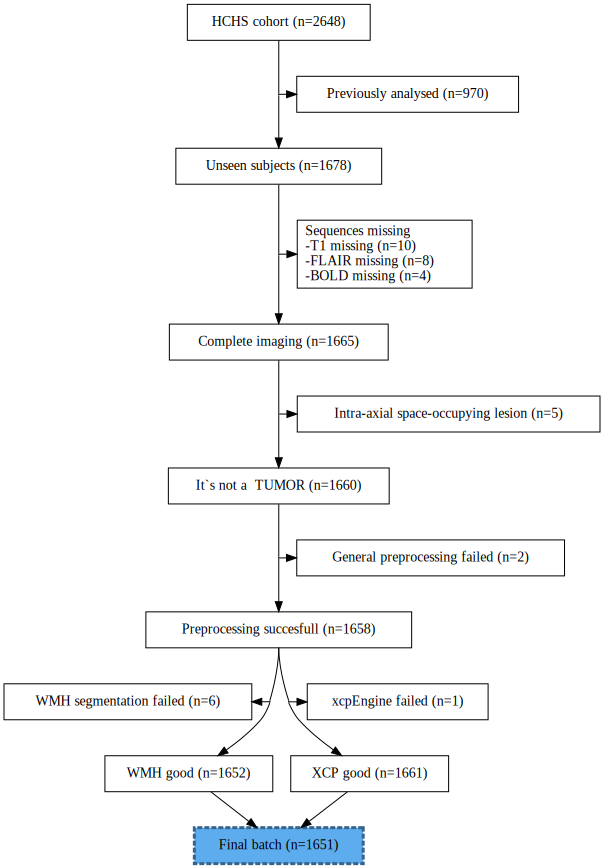
\includegraphics[width=0.5\linewidth]{./../analysis/code/R/FLOW.png}
    \mycaption{Study flowchart}{Composition of the study population after application of inclusion and exclusion criteria, and image processing.}
    \label{fig:flowchart}
\end{figure}




%\addtocounter{table}{-1}
\begin{table}
\centering
\setlength{\LTpost}{0mm}
\begin{longtable}{ll}
\toprule
 & \textbf{N = 1,651} \\ 
\midrule
\emph{Demographics} (no Missing n (\%))\\
\hline
Age, \unit{\year} &  \\ 
\quad Median (IQR) & 66 (59 -- 72) \\ 
Sex &  \\ 
\quad Male & 940/1651 (57\%) \\ 
\quad Female & 711/1651 (43\%) \\ 
\rule{0pt}{3ex}    
\emph{Cardiovascular risk factors}\\
\hline
Hypertension & \\
\quad Present & 1177/1611 (73.1\%) \\
\quad Missing n (\%) & 85 (5.1\%) \\
Diabetes & \\
\quad Present & 157/1566 (10\%)\\
\quad Missing n (\%) & 40 (2.4\%) \\
Smoking & \\ 
\quad Present & 200/1360 (14.7\%) \\
\quad Missing n (\%) & 201 (12.9\%\%)\\
Hyperlipidaemia & \\
\quad Present & 426/1578 (27\%)\\
\quad Missing n (\%) & 73 (4.4\%) \\
\rule{0pt}{3ex}    
\emph{Cognitive test results}\\
\hline
MMSE, \# (max. 30) &  \\ 
\quad Median (IQR) & 28 (27 -- 29) \\ 
\quad Missing n (\%) & 129 (7.8\%) \\ 
Vocabulary (MWT-B), \# (max. 37) &  \\ 
\quad Median (IQR) & 32 (30 -- 34) \\ 
\quad Missing n (\%) & 295 (18\%) \\ 
Word recall, \# (max. 10) &  \\ 
\quad Median (IQR) & 8 (6 -- 9) \\ 
\quad Missing n (\%) & 180 (11\%) \\ 
Animal Naming &  \\ 
\quad Median (IQR) & 24 (20 -- 29) \\ 
\quad Missing n (\%) & 116 (7.0\%) \\ 
TMT-A, seconds &  \\ 
\quad Median (IQR) & 38 (31 -- 48) \\ 
\quad Missing n (\%) & 144 (8.7\%) \\ 
TMT-B, seconds &  \\ 
\quad Median (IQR) & 83 (65 -- 110) \\ 
\quad Missing n (\%) & 162 (9.8\%) \\ 
\rule{0pt}{3ex}    
\emph{History}\\
\hline
Diagnosed dementia & \\
\quad Present & 6/1645 (0.4\%)\\
\quad Missing n (\%) & 6 (0.4\%) \\
Years of education &  \\ 
\quad Median (IQR) & 13 (12 -- 16) \\ 
\quad Missing n (\%) & 34 (2\%) \\ 
\bottomrule
\end{longtable}
\mycaption{Descriptive statistics of the study population}{Data are presented as median (interquartile range) or count (percentage) of non-missing items, as appropriate. Number of percentage of missing items are reported separately.}
\label{tab:democog}
\end{table}


Baseline demographic and cognitive values, including the number of missing items, are reported in \Cref{tab:democog}.

WMH volumes (median \qty{1.05}{\milli\litre}, IQR \qtyrange{0.47}{2.37}{\milli\litre}), motion estimates, and fractional occupancies of brain states 1 through 5 are reported in \Cref{tab:fracocc}. 
\addtocounter{table}{-1}
\begin{table}
\centering
\setlength{\LTpost}{0mm}
\begin{longtable}{ll}
\toprule
& \textbf{N = 1,651} \\ 
\midrule
WMH volume\textsuperscript{1}, \unit{\milli\litre} & \\
\quad Total & 1.05 (0.47 -- 2.37), 9\,Z\\
\quad Periventricular & 0.94 (0.43 -- 2.04), 9\,Z \\
\quad Deep & 0.10 (0.03 -- 0.37), 344\,Z  \\
Motion during rs-fMRI \\
\quad Framewise displacement, \unit{\milli\metre} & 0.21 (0.15 -- 0.63)\\
\quad RMSD, \unit{\milli\metre} & 0.086 (0.058 -- 0.12)\\
\quad DVARS &  27.8 (24.3 -- 31.8)\\
Fractional occupancy, \% \\
\quad DMN+ & 24.8 (20.8 -- 28.0) \\ 
\quad DMN- & 24.0 (20.0 -- 28.0) \\ 
\quad S3 & 18.4 (15.2 -- 22.4) \\ 
\quad S4 & 16.8 (12.8 -- 20.8) \\ 
\quad S5 & 15.2 (12.0 -- 19.2) \\
\bottomrule
\end{longtable}
\textsuperscript{1}Number of zero values indicated by Z
\mycaption{Structural and functional imaging characteristics}{Data are presented as median (interquartile range). Supratentorial WMH volumes were obtained by semiautomatic segmentation of FLAIR images using a BINACA/LOCATE-based $k$-nearest neighbours algorithm and stratified by their distance to the lateral ventricles (<\qty{10}{\milli\metre}, periventricular; >\qty{10}{\milli\metre}, deep). Motion parameters were estimated during fMRIprep processing of BOLD scans. Fractional occupancies were calculated by assigning individual BOLD volumes to one of five discrete brain states defined by k-means clustering-based co-activation pattern analysis.Two high-occupancy states are labelled DMN+ and DMN- in view of their network connectivity profiles as shown in \Cref{fig:spider}.}
\label{tab:fracocc}
\end{table}


In an outcome-neutral quality check of the implementation of (i) the MRI processing pipeline, (ii) brain state estimation, and (iii) co-activation pattern analysis, the mean difference in fractional occupancy between high- and low-occupancy states was consistently maintained, with a point-estimate of the separation between two high-occupancy and three low-occupancy states of \qty{6.7}{\percent} (\qty{95}{\percent} confidence interval, \qtyrange{6.2}{7.1}{\percent}) in the \emph{36p} paradigm. 
This indicates that the implementation of the pipeline was correct and that the brain state estimation and co-activation pattern analysis worked as intended. 


\subsection{Pre-registered hypotheses}
\subsubsection{Association between WMH load and fractional occupancy}
The results of the test of our primary preregistered hypothesis of an association between supratentorial WMH volume and the time spent in high-occupancy brain states are shown in \Cref{fig:hyp1} and \Cref{tab:hyp1}.

\begin{figure}
    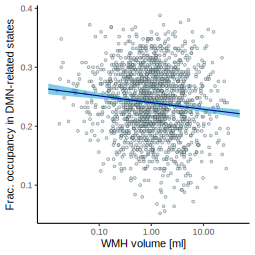
\includegraphics[width=.5\linewidth]{./../analysis/derivatives/Figures/Fig_hyp1.png}
    \mycaption{Association between time spent in high-occupancy brain states and supratentorial WMH volume}{Point estimates (black line) and 95\%-confidence region (light blue ribbon) of the conditional mean fractional occupancy are obtained from unadjusted beta regression modelling. Each marker represents one of N=1642 independent participants with a non-zero total WMH volume. }
    \label{fig:hyp1}
\end{figure}

%\addtocounter{table}{-1}
\begin{table}
\centering
\setlength{\LTpost}{0mm}
\begin{longtable}{lccc}
\toprule
 & Estimate & P & 95\%-CI \\ 
\midrule
Intercept & 0.24 & <0.0001 & 0.21 -- 0.27 \\ 
WMH, per 5.1-fold increase\textsuperscript{1} & 0.94 & <0.0001 & 0.92 -- 0.96 \\ 
Age, per 10 years & 1.04 & 0.001 & 1.01 -- 1.06 \\ 
Female sex & 1.12 & <0.0001 & 1.09 -- 1.16 \\ 
$\mathbf{1}_{\{\operatorname{WMH=0}\}}$ & 0.93 & 0.477 & 0.75 -- 1.14 \\ 
\bottomrule
\end{longtable}
\textsuperscript{1} Interquartile ratio $2.37/0.468=5.06$
\mycaption{Association between time-spent in high-occupancy DMN-related brain states and WMH adjusted for age and sex}{Beta regression table estimated from $n=1651$ independent participants using the model equation $\operatorname{FO}^{\text{high}} \sim \log{\operatorname{WMH}^+} + \mathbf{1}_{\{\operatorname{WMH=0}\}} + \operatorname{age} + \operatorname{sex}$.}
\label{tab:hyp1}
\end{table}


Adjusted for age and sex, there was a \num{0.94}-fold reduction in the odds of occupying a high-occupancy brain state for every \num{5.1}-fold increase in WMH load (P \num{5.01e-8}).

\subsubsection{Association between executive function and fractional occupancy in DMN-related states}

The results of the test of our secondary preregistered hypothesis of an association between time spent in high-occupancy brain states and executive function as measured by the complete part B of the TMT are shown in \Cref{fig:hyp2} and \Cref{tab:hyp2}.

\begin{figure}
    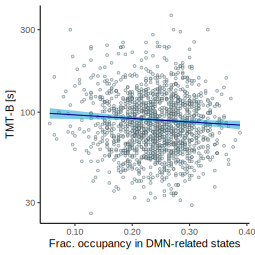
\includegraphics[width=.5\linewidth]{./../analysis/derivatives/Figures/Fig_hyp2.png}
    \mycaption{Association between time spent in high-occupancy DMN-related brain states and TMT-B completion time}{Point estimates (black line) and 95\%-confidence region (light blue ribbon) of the conditional mean TMT-B completion time are obtained from unadjusted Gamma regression modelling. Each marker represent one of N=1482 independent participants with non-zero total WMH volume and available TMT-B data.}
    \label{fig:hyp2}
\end{figure}

%\addtocounter{table}{-1}
\begin{table}
\setlength{\LTpost}{0mm}
\begin{longtable}{lccc}
\toprule
 & Estimate & P & 95\%-CI \\ 
\midrule
Intercept & 53.41 & $<0.0001$ & 42.7 -- 66.8 \\ 
$\operatorname{FO}^{\text{high}}$, per 5\% & 0.98 & 0.0116 & 0.96 -- 0.99 \\ 
WMH, per 5.1-fold increase\textsuperscript{1} & 1.01 & 0.367 & 0.98 -- 1.05 \\ 
Age, per 10 years & 1.18 & <0.0001 & 1.15 -- 1.21 \\ 
Female sex & 0.99 & 0.666 & 0.95 -- 1.03 \\ 
Education, per year & 0.97 & <0.0001 & 0.97 -- 0.98 \\ 
$\mathbf{1}_{\{\operatorname{WMH=0}\}}$ & 0.97 & 0.398 & 0.92 -- 1.03 \\
\bottomrule
\end{longtable}
\textsuperscript{1} Interquartile ratio $2.37/0.468=5.06$
\mycaption{Association between TMT-B and time spent in high-occupancy DMN-related brain states adjusted for age, sex, WMH volume and years of education}{Gamma regression table estimated from $n=1483$ independent participants using the model equation $\operatorname{TMT-B} \sim \operatorname{FO}^{\text{high}} + \log{\operatorname{WMH}^+} + \mathbf{1}_{\{\operatorname{WMH=0}\}} + \operatorname{age} + \operatorname{sex} + \operatorname{educationyears}$.}
\label{tab:hyp2}
\end{table}

Adjusted for age, sex, WMH volume, and years of education, there was a \num{0.98}-fold reduction in the time to complete the TMT-B for every \qty{5}{\percent} increase in the time spent in high-occupancy brain states (P \num{0.0116}).


\subsection{Multiverse analysis}

In a multiverse analysis, the main findings of associations between WMH load and FO and, to a lesser extent, between FO and TMT-B were robust with respect to the processing choices of brain parcellation and confound regression strategy.

A nominally statistically significant negative association between the total WMH load and time spent in high-occupancy states was observed in 48/81 scenarios, with 8/81 significant positive associations occurring with the Desikan--Killiany parcellation only (\Cref{fig:mv}{A}). 
For periventricular (deep) WMH volume, the results were similarly robust with 49/81 (39/81) negative and 8/81 (0/81) positive associations of nominal statistical significance, respectively.

The secondary finding of an association between greater TMT-B times and lower fractional occupancy was less robust with only 16/81 nominally statistically significant negative and no significant positive associations, irrespective of operationalization of cSVD (total vs. periventricular vs. deep WMH volume) (\Cref{fig:mv}{B}).

\begin{figure}
    \includegraphics[width=\linewidth]{./../analysis/derivatives/Figures/Fig_mv.png}
    \mycaption{Multiverse analysis}{Adjusted effect size estimates of the associations between cSVD severity (WMH volume) and network dedifferentiation (less time spent in high-occupancy DMN-related brain states) [\textbf{A)}], and between network dedifferentiation and executive function (TMT-B completion time) [\textbf{B)}]. Effect sizes are given per 5.1-fold increase in WMH volume and a 5\%-increase in fractional occupancy, respectively. Markers and line segments indicate point estimates and 95\%-confidence intervals for adjusted odds ratios for different combinations of confound regression strategy and brain parcellation. The primary analytical choices are indicated by dark blue circles (\emph{}36p) and light blue shading (Schaefer-400). Model equations for beta and gamma regressions, respectively, are given at the top. Vertical lines indicate no effect (black) and the effect size observed in the discovery cohort \citep{Schlemm2022-he} (light blue), respectively, for reference. Effect sizes not reaching nominal statistical significance ($\alpha=0.05$) are shown desaturated. Corresponding data based on periventricular and deep WMH volumes are presented in the Supplementary Appendix.}
    \label{fig:mv}
\end{figure}

\subsection{Additional analyses}
\subsubsection{Connectivity profiles of brain states -- relation to default mode network}
Based on the cosine similarity between positive and negative activations of cluster centroids and indicator vectors of pre-defined large scale brain networks, network activation profiles were computed for brain states estimated from Schaefer parcellations of varying spatial resolutions.

\Cref{fig:spider} shows the corresponding spider plots, identifying states characterized by activation (DMN+) or suppression (DMN-) of the default mode network as states with the highest fractional occupancy.

\begin{figure}
    %\begin{subfigure}{1.0\textwidth}
    \includegraphics[width=\linewidth]{./../analysis/derivatives/Figures/surface/surfaces.png}
    \includegraphics[width=\linewidth]{./../analysis/derivatives/Figures/spiderplot_36p~schaefer400x7.png}
    %\caption{Spider400}
    %\label{fig:spider400}
    %\end{subfigure}
    % \begin{subfigure}{1.0\textwidth}
    % \includegraphics[width=\linewidth]{./../analysis/derivatives/Figures/spiderplot_36p~schaefer200x7.png}
    % \caption{Spider200}
    % \label{fig:spider200}
    % \end{subfigure}
    % \begin{subfigure}{1.0\textwidth}
    %     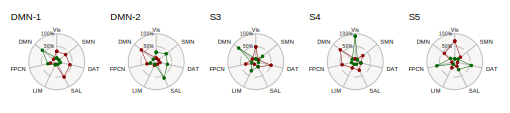
\includegraphics[width=\linewidth]{./../analysis/derivatives/Figures/spiderplot_36p~schaefer100x7.png}
    %     \caption{Spider200}
    %     \label{fig:spider100}
    %     \end{subfigure}
    \mycaption{Connectivity profiles of brain states}{[\textbf{Top}] Centroids of each identified brain state visualized in brain space. Note the individual color scales. [\textbf{Bottom}] Cosine similarity between centroids of brain states and signed indicator vectors corresponding to activation (green) and suppression (red) of each of seven predefined large-scale functional brain networks \citep{Yeo2011-qg}. 
    
    States are ordered by mean fractional occupancy across N=1651 independent participants, indicated by parenthetical percentages. Two high-occupancy states are characterized by activation or suppression of the DMN, the remaining three low-occupancy states (S3--5) were not used in the present study. Note that mean FO values are similar, but not identical, to median FO values reported in \Cref{tab:fracocc}.}
    \label{fig:spider}
\end{figure}


\subsubsection{Association with other cognitive domains}
Associations between the time spent in high-occupancy DMN-related brain states and cognitive measures beyond TMT-B are shown in \Cref{fig:FOvsCOG}.

\begin{figure}
    \includegraphics[width=\linewidth]{./../analysis/derivatives/Figures/Fig_FOvsCOG.png}
    \mycaption{Association between time spent in high-occupancy DMN-related brain states and cognitive measures}{Point estimates (black line) and 95\%-confidence region (light blue ribbon) of the conditional mean cognitive measures are obtained from unadjusted binomial (top row: Mini-Mental State Examination, Vocabulary, Word List Recall, logit link) and Gamma regression (bottom row: Animal Naming, Trail Making Test [TMT] A/B: log link) modelling. 
    
    Each marker represents one of N independent participants, as indicated. Insets report effect sizes and P-values both with (adjusted [a-]) and without adjustment for the nuisance variables age, sex, WMH volume (coded as in \Cref{fig:mv}), and years of education. Effect sizes were quantified as odds ratios (ORs) (top) or response scale multipliers [exp(b)] (bottom), and correspond to a 20\%-increase in fractional occupancy. Note the different reference change in FO compared to \Cref{tab:hyp2} chosen to adequately represent some of the smaller effect sizes. The bottom right panel highlighted in dark blue reproduces \Cref{fig:hyp2}.}
    \label{fig:FOvsCOG}
\end{figure}


Adjusted for age, sex, WMH load, and years of education, FO in DMN-related states appeared to be associated with better word recall (adjusted OR 1.19, nominal P 0.013), but not with global cognitive functioning (MMSE, adjusted OR 1.09) or vocabulary (aOR 1.09), nor with verbal fluency (animal naming, adjusted $\exp(\beta)$ 1.04), or pure processing speed (TMT-A, adjusted $\exp(\beta)$ 0.97).